\documentclass[10pt,aspectratio=169]{beamer}

% All the boilerplate is in ccaslides.sty
% Note that this also pulls in a custom vogtwidebar.sty
\usepackage{ccaslides}

\author{Ji\v{r}\'i Lebl}

\institute[OSU]{%
Departemento pri Matematiko de Oklahoma {\^S}tata Universitato}

\title{Cultivating Complex Analysis:\\%
The Riemann sphere (1.3)}

\date{}

\begin{document}

\begin{frame}
\titlepage
\end{frame}

\begin{frame}
Real numbers are sometimes extended to add $\pm \infty$.

\medskip
\pause

Similarly, the complex plane is extended by adding $\infty$ (only one
infinity):
\[
\C_{\infty} = \C \cup \{ \infty \} .
\]

\pause
We call $\C_{\infty}$ the \emph{Riemann sphere}.

\medskip
\pause

To define topology, define a bijection $g \colon \C_\infty \to \C_\infty$ by
\[
g(z) =
\begin{cases}
\nicefrac{1}{z} & \text{if } z \not= 0 \text{ and } z \not= \infty, \\
\infty & \text{if } z = 0, \\
0 & \text{if } z = \infty.
\end{cases}
\]

\pause

We want all open sets in $\C$ to be open in $\C_\infty$.

\medskip
\pause

Neighborhoods of $\infty$ are $g(U)$ for neighborhoods $U$ of $0$.

\medskip
\pause

If talking about convergence at $z \in \C$, we just use the normal
topology.

\medskip
\pause

If talking about convergence at $\infty$, we map with $g$
and consider the topology at $0$.
\end{frame}

\begin{frame}
We can give $\C_\infty$ a metric space structure through the
\emph{stereographic projection}:

\medskip
\pause

Let $S^2$ be the unit sphere in $\R^3$.  We define
a bijection $\Phi \colon S^2 \to \C_{\infty}$.

\medskip
\pause

Start with $\Phi\bigl((0,0,1)\bigr) = \infty$.

\medskip
\pause

%$(x,y) = x+iy \in \R^2=\C$  is identified

For any $p \in S^2 \setminus (0,0,1)$ there is a unique
line through $(0,0,1)$ and $p$.

\medskip
\pause

The line intersects the $xy$-plane at a unique point $(x,y,0)$.

\medskip
\pause

We identify $(x,y,0)$ with $\xi=x+iy$ and define
$\Phi(p) = \xi$.

\medskip
\pause

\begin{center}
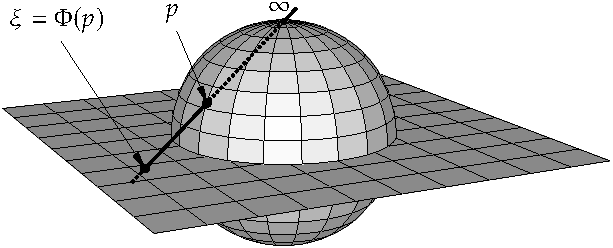
\includegraphics[width=3.6in]{../figures/riemannsphere}
\end{center}

\end{frame}

\begin{frame}
%One can give an explicit formula (exercise) for $\Phi$, for example in
%spherical coordinates on $S^2$, $(\phi,\theta)$ (zenith,azimuth),
%$\Phi$ takes $(\phi,\theta)$ to $\cot(\nicefrac{\phi}{2})e^{i\theta}$.
%
%\medskip
%
The point of the Riemann sphere is to give the value $\infty$ to certain
limits and to allow limits as $z$ tends to $\infty$.

\medskip
\pause

Note that conveniently
$\C_\infty$ is compact (one-point compactification of $\C$)

\medskip
\pause
For $f \colon U \subset \C_\infty \to \C_\infty$, define
\begin{equation*}
\lim_{z \to z_0} f(z) = L
\end{equation*}
using the topology of the Riemann sphere.

\medskip
\pause

It is an exercise to show the following:

\medskip
\pause

$L \in \C$ and $z_0 \in \C$: \quad
$\lim\limits_{z\to z_0} f(z) = L$ in $\C_\infty$ 
$\Leftrightarrow$ $\lim\limits_{z \to z_0} f(z) = L$ in $\C$.

\medskip
\pause
$L \in \C$: \quad
$\lim\limits_{z\to \infty} f(z) = L$ in $\C_\infty$
$\Leftrightarrow$ $\forall$ $\epsilon > 0$ $\exists$ $M$ such that
$\sabs{f(z)-L} < \epsilon$ whenever $\sabs{z} > M$.

\medskip
\pause
$z_0 \in \C$: \quad
$\lim\limits_{z\to z_0} f(z) = \infty$ in $\C_\infty$
$\Leftrightarrow$ $\forall$ $M > 0$ $\exists$ $\delta > 0$ such that
$\sabs{f(z)} > M$ whenever $\sabs{z-z_0} < \delta$.

\medskip
\pause

$L \in \C_\infty$: \quad
$\lim\limits_{z\to\infty} f(z) = L$ $\Leftrightarrow$
$\lim\limits_{z \to 0} f(\nicefrac{1}{z}) = L$.

\medskip
\pause

$z_0 \in \C_\infty$: \quad
$\lim\limits_{z\to z_0} f(z) = \infty$ $\Leftrightarrow$
$\lim\limits_{z \to z_0} \frac{1}{f(z)} = 0$.
\end{frame}

\begin{frame}
It makes sense to talk about the value of $\nicefrac{1}{z}$ at the origin
as $\infty$, and the value of $z$ at $\infty$ as $\infty$.

\medskip
\pause

Consider a polynomial $P(z) = a_d z^d + a_{d-1} z^{d-1} + \cdots + a_1 z +
a_0$.

\medskip
\pause

If $d \geq 1$ and $a_d \not= 0$, then it is an exercise to show that
\[
\lim_{z \to \infty} P(z) = \infty
\]
\pause
To see it, prove that for large $z$, $\abs{P(z)} \geq c \abs{z}^d$
for some $c$.

\medskip
\pause

So every nonconstant polynomial is $\infty$ at $\infty$.

\medskip
\pause

\textbf{Remark:}
Be careful about limits in extended real sense vs. Riemann sphere sense:
\begin{equation*}
\lim_{x \to 0} \frac{1}{x} \quad \text{does not exist,} \qquad \text{but} \qquad
\lim_{z \to 0} \frac{1}{z} = \infty .
\end{equation*}
(if we think of $x$=real, and $z$=complex)

\medskip
\pause

We'll use Riemann sphere sense unless otherwise noted or obvious.
We may use $+\infty$ to distinguish from Riemann sphere $\infty$
if confusion could arise.
\end{frame}

\begin{frame}
Partial arithmetic can be defined on $\C_\infty$:

\medskip
\pause

If $c \not= \infty$, declare $c+\infty = \infty$.

\medskip
\pause

Neither $\infty+\infty$ nor $\infty-\infty$ makes sense:

if $f(z) = z$ and $g(z) = -z$,
then $\lim\limits_{z \to \infty} f(z) = \infty$,
$\lim\limits_{z \to \infty} g(z) = \infty$, but $\lim\limits_{z \to \infty}
\bigl(f(z)+g(z)\bigr) = 0$.

\medskip
\pause

If $c \not= 0$, then define $\nicefrac{c}{0} = \infty$ and $c \cdot \infty =
\infty$.

\medskip
\pause

If $c \not= \infty$, then define $\nicefrac{c}{\infty} = 0$.

\medskip
\pause

$0 \cdot \infty$, $\nicefrac{0}{0}$, and $\nicefrac{\infty}{\infty}$ are undefined.

\medskip
\pause

Note that this is different from the extended real arithmetic.

\end{frame}

\end{document}
